\chapter{Přiříz architecture and requirements}\label{architecture}

	Previous chapters should provide enough information to understand basic principles of a RESTful service and benefits of
	using BPM. Discussion about the two mentioned will become more concrete from now on, because admission process will be
	taken into account.
	
	As a result of this master's thesis a working application is implemented. Further referred as \textbf{RESTful API} and
	it integrates both technologies.
	 	
	This chapter describes requirements for application functionality and its role in the architecture of the whole project
	currently running at CTU FIT.

	\section{\gls{FIS}}
	
	The project covers activities related to information system development CTU. It is quite complicated and long term
	project involving more than dozen people in various roles. RESTful API with two other applications directly
	interconnected is just a part of it and together they form \textbf{Přiříz} component \ref{fig:fis_architecture}.
	
	\newpage
	\begin{figure}[h]
		\label{fig:fis_architecture}
	  	\centering
	    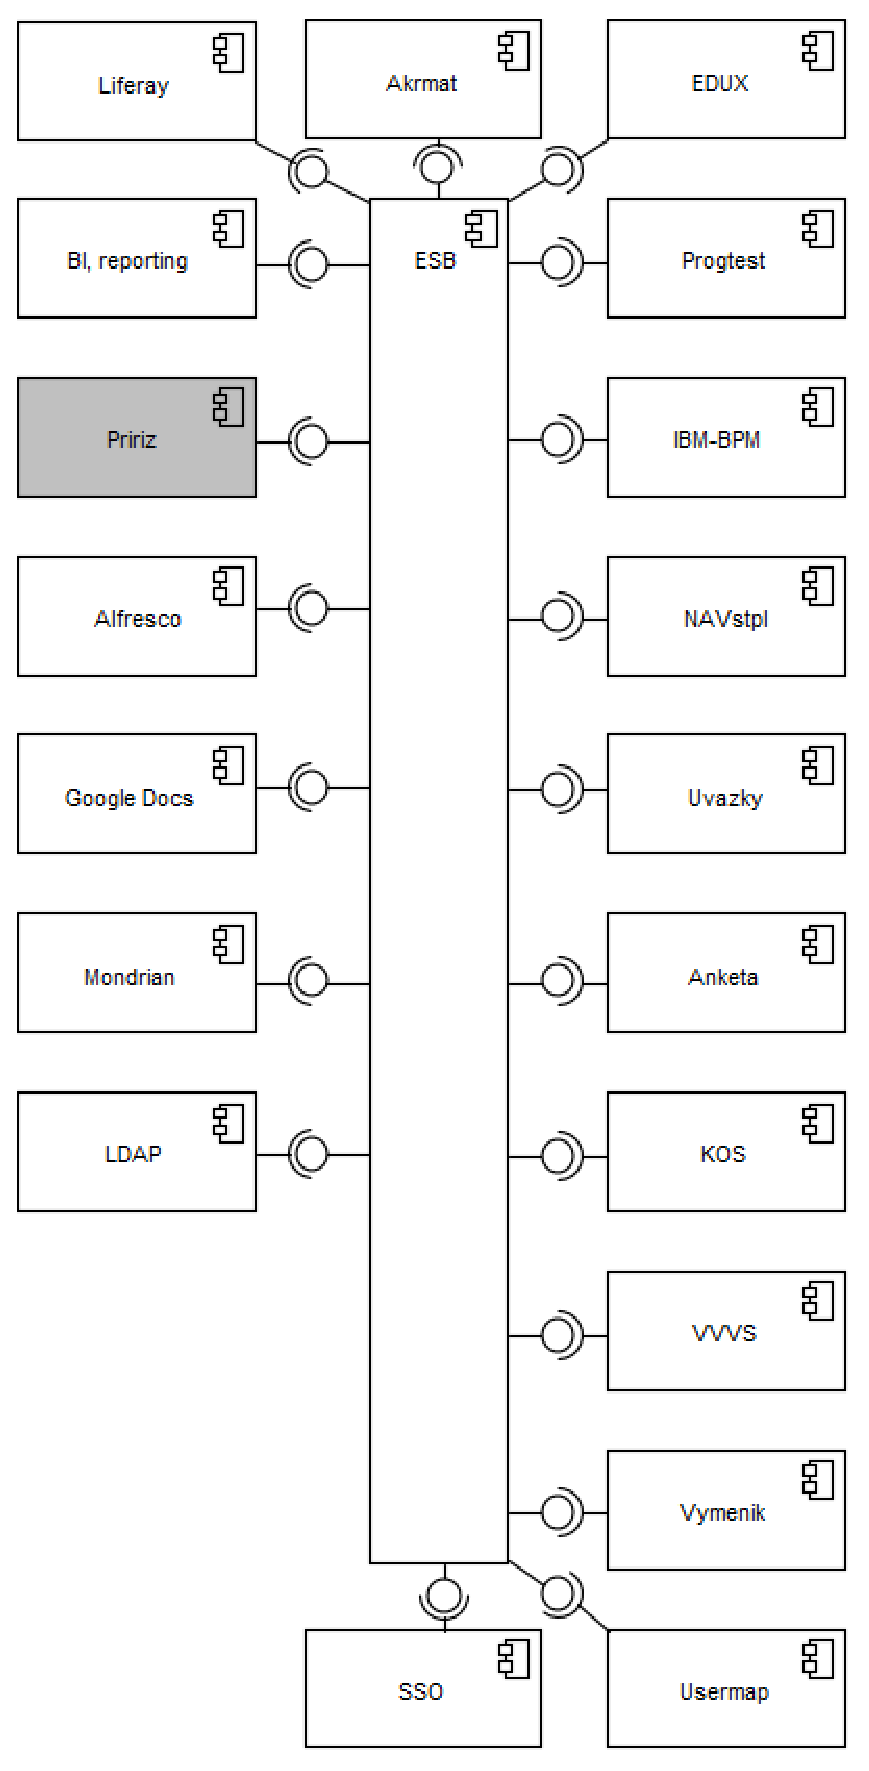
\includegraphics[width=6cm]{figures/fis_architecture}
	  	\caption{FIS architecture}
	\end{figure}
	
	\section{Catalogue of requirements}
	
	This section lists requirements for the RESTful API. 
	
	\subsection{Functional requirements}
	
	Functional requirements define which services should system provide. 
	\begin{itemize}
		\item F00 Admission import
	
		data import from e-admission, on-line CTU form
		
		\item F01 Admission evidence
	
		evidence of valid admissions
		
		\item F01.1 Admission detail
		
		detailed information about admission and admissioner
		
		\item F01.2 Admission edit
		
		update of allowed admission data
		
		\item F01.3 Password reset
		
		allow password reset/recovery to a valid user account related to the admission
	
		\item F02 Term evidence
	
		entrance exam term evidence
		
		\item F02.1 Term management
		
		entrance exam term management
		
		\item F02.2 Enrollment term management
	
		enrollment term of accepted admissioners management
		
		\item F02.3 Term registrations evidence
	
		Entrance exam or enrollment term registrations of admissionsers evidence
	
		\item F03 Statistics
	
		various statistics of this year's admission process
	
		\item F04 User management
	
		password change
	
		\item F05 Admission state
	
		view current state of admission
		
		\item F05.1 Entrance exam registration
		
		allow an admissioner to book entrance exam term
		
		\item F05.2 Entrance exam apology
		
		allow an admissioner to apologise from the entrance exam registration
		
		\item F05.3 Enrollment registration
		
		allow an admissioner to book enrollment term
		
		\item F05.4 Enrollment apology
		
		allow an admissioner to apologise from the enrollment registration
		
		\item F06 Admission process management
		
		allow management of an admission during admission process
		
		\item F06.1 Send e-mails
		
		allow sending of informative e-mail
		
		\item F06.2 User action processing
		
		allow processing of user actions during admission process
		
		\item F07 File number administration
		
		allow file number assignment to documents communicated with an admissioner
		
		\item F08 Document creation
		
		allow document creation of various types for an admissioner 
	\end{itemize}
	
	\subsection{Non-functional requirements}
	
	Non-functional requirements do not directly define system functionality, but describe constraints or general
	properties.
	
	\begin{itemize}
		\item NF01 User action processing
	
		jBPM engine requires local TaskService server to handle user actions in process
		
		\item NF02 E-mail server configuration

		jBPM engine requires properly configured mail sender to be able to use CTU's mail server
		
		\item NF03 Technologies
		
		use the following for implementation: JEE, Apache Maven, jBPM, Spring Framework, Spring Roo, JPA
		
		\item NF04 System and web service security
		
		system and web services will be secured
		
		\item NF04.1 User roles and permissions
		
		security will be handled by user roles and permissions
		
		\item NF05 MySQL database
		
		primary DBMS will be MySQL
		
		\item NF06 Server Tomcat
		
		RESTful API will be able run on Apache Tomcat servlet container
		
		\item NF07 Performance under load
		
		system must handle 250 concurrent users and 2500 total users
		
		\item NF07.1 Scaling
		
		system must be able to split load among multiple instances
	\end{itemize}
	
	During the development process several changes were made to the catalogue of requirements. RESTful API team and UI team
	switched responsibilities for  F07, F08. F03 was descoped but can be implemented when needed.
	
	NF07.1 is a matter of infrastructure. While this work was being created, only one virtual server was available for the
	whole Přiříz project and makes no sense to configure multiple instances on a single machine.
